\section{Secure Communication}

\begin{frame}{Events and Notifications}
\begin{itemize}
\item Keeping it simple: \texttt{SecureCommunication} is a passive component
\item \texttt{NetworkStack\_PicoTcp} component uses \texttt{run()} routine to notify clients about new events
\item \textbf{Problem:}  No \texttt{run()} loop = No notifications = Calls like \texttt{OS\_Socket\_wait()} don't work anymore
\item \textbf{Solution:} Merge functionality of \texttt{OS\_Socket\_wait()} with \texttt{OS\_Socket\_connect()}
    \begin{itemize}
    \item In our usecase, \texttt{OS\_Socket\_wait()} was only called to make sure we received an event confirming the successful establishment of a connection
    \end{itemize}
\end{itemize}
\end{frame}

\begin{frame}{Key Exchange}
\begin{itemize}
\item Key exchange must happen before sending/receiving any other data
\item \textbf{Problem:} How do we synchronize \texttt{SecureCommunication} with the client component?
\item \textbf{Solution:} A socket must always be created before you can read/write data on it.
    \begin{itemize}
    \item Static variable in \texttt{SecureCommunication} keeps track of whether the key has been exchanged already.
    \item Inside the code called by \texttt{OS\_Socket\_create()}, check the value of that variable, exchange key if necessary before creating socket and returning.
    \end{itemize}
\end{itemize}
\end{frame}

\begin{frame}{Encryption and Decryption Protocol}
\begin{itemize}
\item Previously in the homeworks: static IV
\item \textbf{Problem:} Using a repeated IV is unsafe!
\item \textbf{Solution:} Append a fresh IV to the beginning of every message
\end{itemize}
\centering
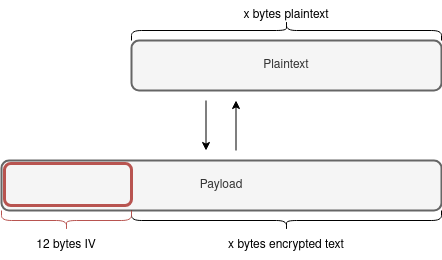
\includegraphics[height = 3.5cm]{payload.png}
\end{frame}